\documentclass{article}
\usepackage{graphicx}
\usepackage{subfigure}
\usepackage{longtable}
\usepackage{latexsym}
\usepackage{amsmath}
\usepackage{subfig}
\usepackage{amssymb}
\usepackage{geometry}
\usepackage{minipage-marginpar}
\usepackage{float}
\geometry{bottom=2.5cm}
\begin{document}
\title{Rapid Prototyping Computer System Report\\Software Infrastructure Group}
\author{Wanjun Xu, Wenjia Liu, Anjie Wang, Hanxiang Ren}
\date{\today}
\maketitle

\newpage

\tableofcontents

\newpage

\section{Function Requirements}

\subsection{Challenge}
 The Children’s School at CMU challenged the Rapid Design and Prototyping for Computer systems class to:
\begin{itemize}
	\item Help track the locations and activities of all members of the school 
	\item Help make dismissal an easier and less stressful process 
\end{itemize}

The whole class discussed together and had a vision scenario. According to the Human Computer Interaction Group, we have known the functions we need to implement and the other requirements we have to complete for connections with other group.

\subsection{Functional Requirements}
\subsubsection{Client Requirements}
\begin{enumerate}
	\item Show the information to the parents and the teachers
	\item Provide user control, for example: log in/out
	\item Provide message service, send and receive message or notification between teachers and parents 
	\item Show the result of data analysis, or the graph of data visualization
	\item Provide a list of children need to be dismissed to teachers
\end{enumerate}

\subsubsection{Implementation Requirements}
Our group member compared the mainstream database, programming language, server and decided the ones which suit the situation most. 

\begin{enumerate}
	\item Read and send data from database
	\item Provide API to Data Visualization Group to show the result
\end{enumerate}


\section{Feature Comparison}
Our group member compared the mainstream database, programming language, server and decided the ones which suit the situation most. 
\subsection{Database}

\begin{table}[htbp]
\centering
  \begin{tabular}{|l|l|p{2cm}|p{2cm}|p{2cm}|p{2cm}|}
  \hline
   Database & Cost & Platform & Company & Language & Character\\
    \hline
   SQLite & Free & Windows, Linux, Unix & D. RichardHipp & Tcl, C\#, PHP, Java & Small, Fast\\
    \hline

   MySQL & Free & Windows, Linux, Unix & MySQL AB & PHP, Perl, Python & Open source, Small, Mediocre online support \\
       \hline

   Oracle & Expensive & Windows, Linux, Unix & Oracle & &\\   
       \hline
	SQL Server & \$931 & Windows, Linux, Unix & Microsoft & XML & Safe, Efficient, Smart, Big \\
	\hline
     \end{tabular}
  \caption{Database Comparison}
\end{table}

SQLite is very small and fast. So it is very good for a mobile phone. Besides, SQLite can be applied to WEB and APP, which others can’t. Finally we choose SQLite.

\subsection{Programming Language}
Each of us have different skills. So we divide the work into PC, APP and website. We use C\# to make a executable program in PC, use Java to make APP and use HTML, css, JavaScript to make the website.

\begin{table}[htbp]
\centering
  \begin{tabular}{|l|p{2cm}|p{2cm}|p{2cm}|p{2cm}|}
  \hline
   Language(Framework) & MVC Framework & Testing Framework & Security Framework & Licence\\
    \hline
   C++(CppCMS) & Yes & No & Yes & MIT\\
    \hline

   Spring & Yes & Mock Objects, Unit tests & Spring Security & Apache 2.0\\
       \hline

   Python(Django) & Yes & Yes & Yes & BSD \\   
	\hline
     \end{tabular}
  \caption{Programming Language Comparison}
\end{table}

\subsection{Server}
Cloud Server is maintained by professional team, thus has better Security. However, a PC owned by child school can bear almost all of the tasks and it's free. So we select Local server, since it could fulfill our demands, and is much cheaper.

\begin{table}[htbp]
\centering
\begin{tabular}{|l|l|l|l|}
	\hline
	Server Type & Price & Storage & Security \& Stability \\
	\hline
	Local Server & ¥15k(New Server)/Free(PC) & Local Hard Disk & Fair \\
	\hline
	Cloud Server & ¥22.50/M & ¥0.24/GB/M & High \\
	\hline
	
\end{tabular}
	\caption{Server Comparison}
\end{table}

\section{Implementations \& Various Ends}
We designed various ends to fulfill different demand. We will first explain details of implementation for each function requirement, and then show interfaces of each end.

\subsection{Login}
Different users have different different levels of authority. Software stores user information in database, retrieve them when users login, finally redirect to different dashboard page based on their identity.

 	\begin{figure}[H] 	
 		\begin{minipage}[b]{0.28\linewidth}
		 	\centering
	 		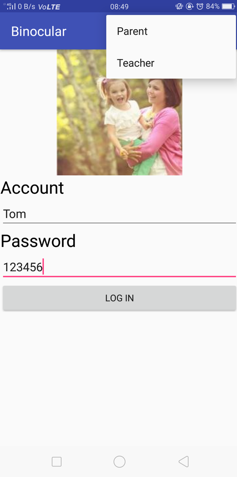
\includegraphics{img/login2.png}
 			\caption{Android End}
 		\end{minipage}
 		\begin{minipage}[b]{0.68\linewidth} 		
 	 		\centering
 			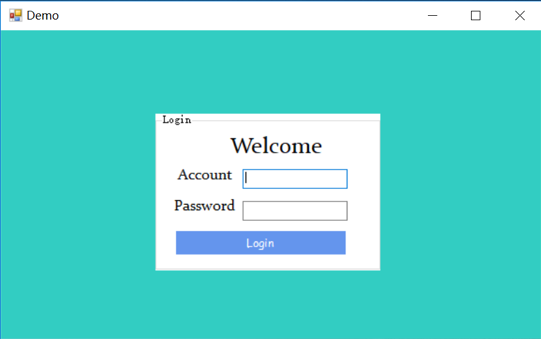
\includegraphics{img/login3.png}
 			\caption{PC End}
	 	\end{minipage}
 	\end{figure}
 	
 	 \begin{figure}[H]
 	 \centering
 		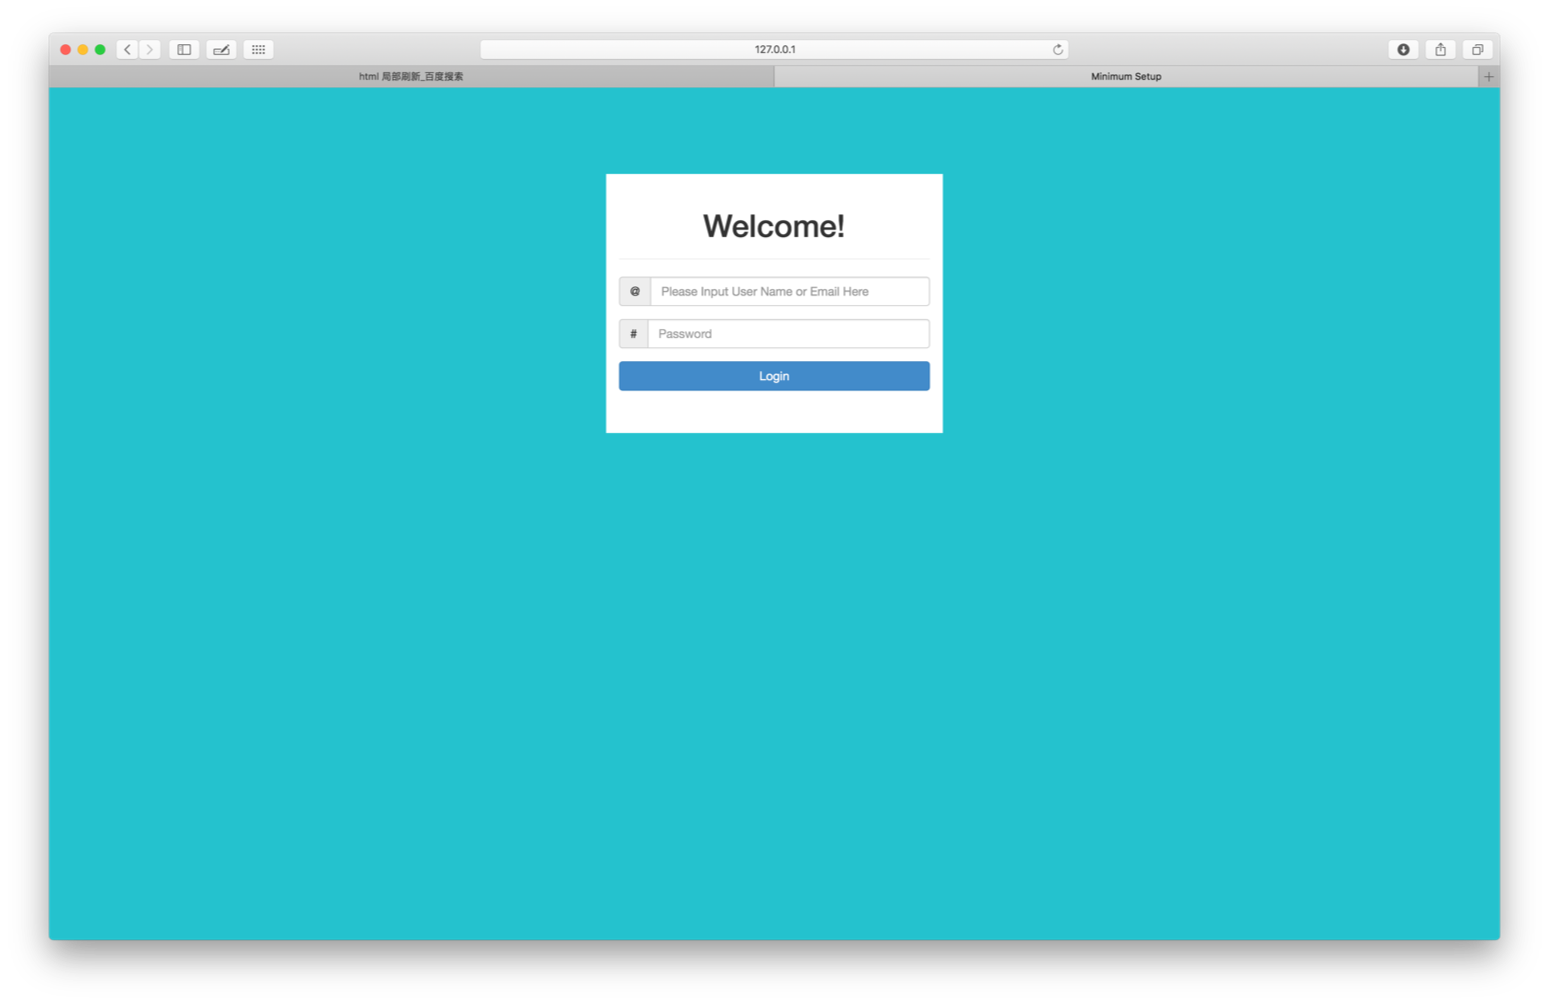
\includegraphics[width=\linewidth]{img/login1.png}
 		\caption{Web End}
 	\end{figure}
 
\subsection{Dashboard}
This page displays tables and graphs generated by data visualization group. Web end application uses JavaScript. Script runs when page loads, and displays graphs on the webpage.
 	\begin{figure}[H] 	
 		\begin{minipage}[b]{0.28\linewidth}
		 	\centering
	 		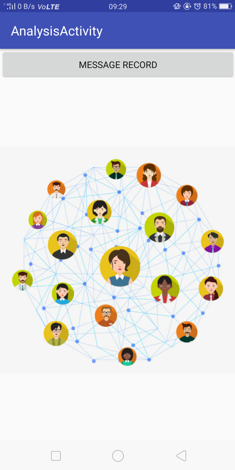
\includegraphics{img/social3.png}
 			\caption{Android End}
 		\end{minipage}
 		\begin{minipage}[b]{0.68\linewidth} 		
 	 		\centering
 			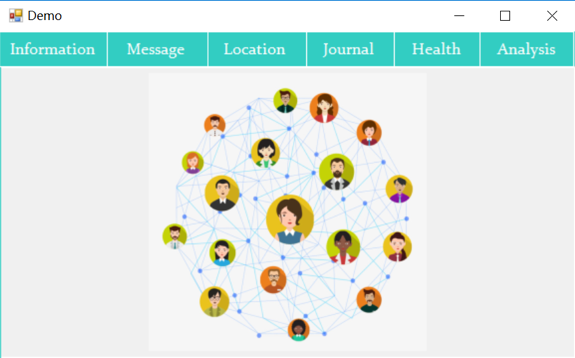
\includegraphics{img/social1.png}
 			\caption{PC End}
	 	\end{minipage}
 	\end{figure}
 	
 	 \begin{figure}[H]
 	 \centering
 		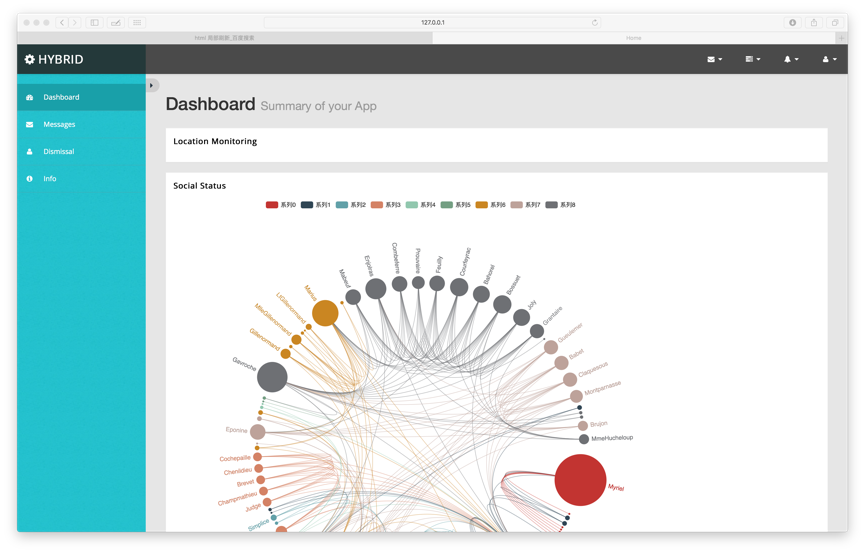
\includegraphics[width=\linewidth]{img/social2.png}
 		\caption{Web End}
 	\end{figure}
 	
\subsection{Dismissal}
Dismissal is a dynamic queue showing children to be dismissed. Dismissal team get notified when parents arrive at parking lot, and a message containing plate number, and parent information will be written into database. Our software read message from database and display corresponding child name on the screen. When a child arrive at waiting area, a sensor detects the child's arrival and write another message containing child's information into database. The software then marks the child as 'Picked up' and remove him/her from the list.
 	\begin{figure}[H] 	
 		\begin{minipage}[b]{0.28\linewidth}
		 	\centering
	 		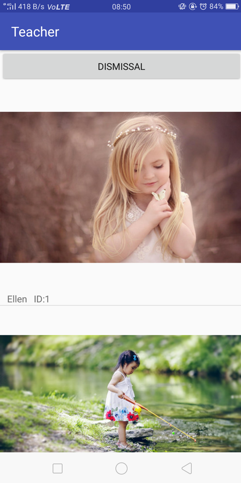
\includegraphics{img/dismissal1.png}
 			\caption{Android End}
 		\end{minipage}
 		\begin{minipage}[b]{0.68\linewidth} 		
 	 		\centering
 		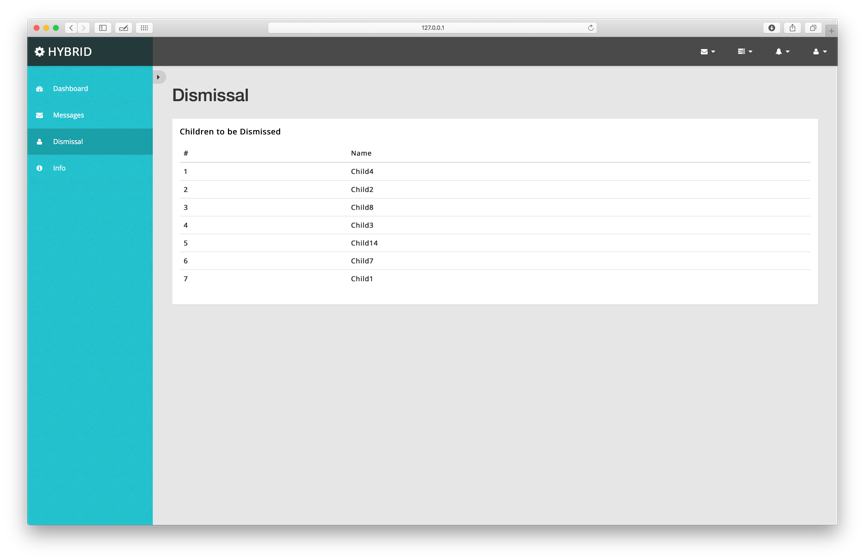
\includegraphics[width=\linewidth]{img/dismissal2.png}
 		\caption{Web End}
	 	\end{minipage}
 	\end{figure}
 	

\subsection{Message}
The message modular allow parents and teachers to communicate through the software, exchanging the information of the children. When a user send a message to anothor user, the message will be stored in the datebase. And when a user enter the message page, the software will fetch messages sent to him/her from the database and show them in the page.
	\begin{figure}[H]
 	 \centering
 		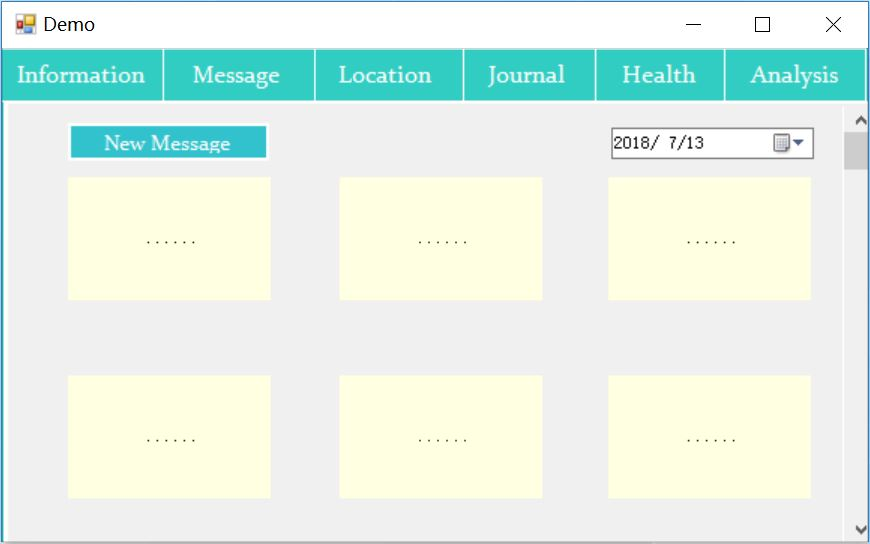
\includegraphics[width=0.8\linewidth]{img/message1.png}
 		\caption{PC End}
 	\end{figure}
 	\begin{figure}[H]
 	 \centering
 		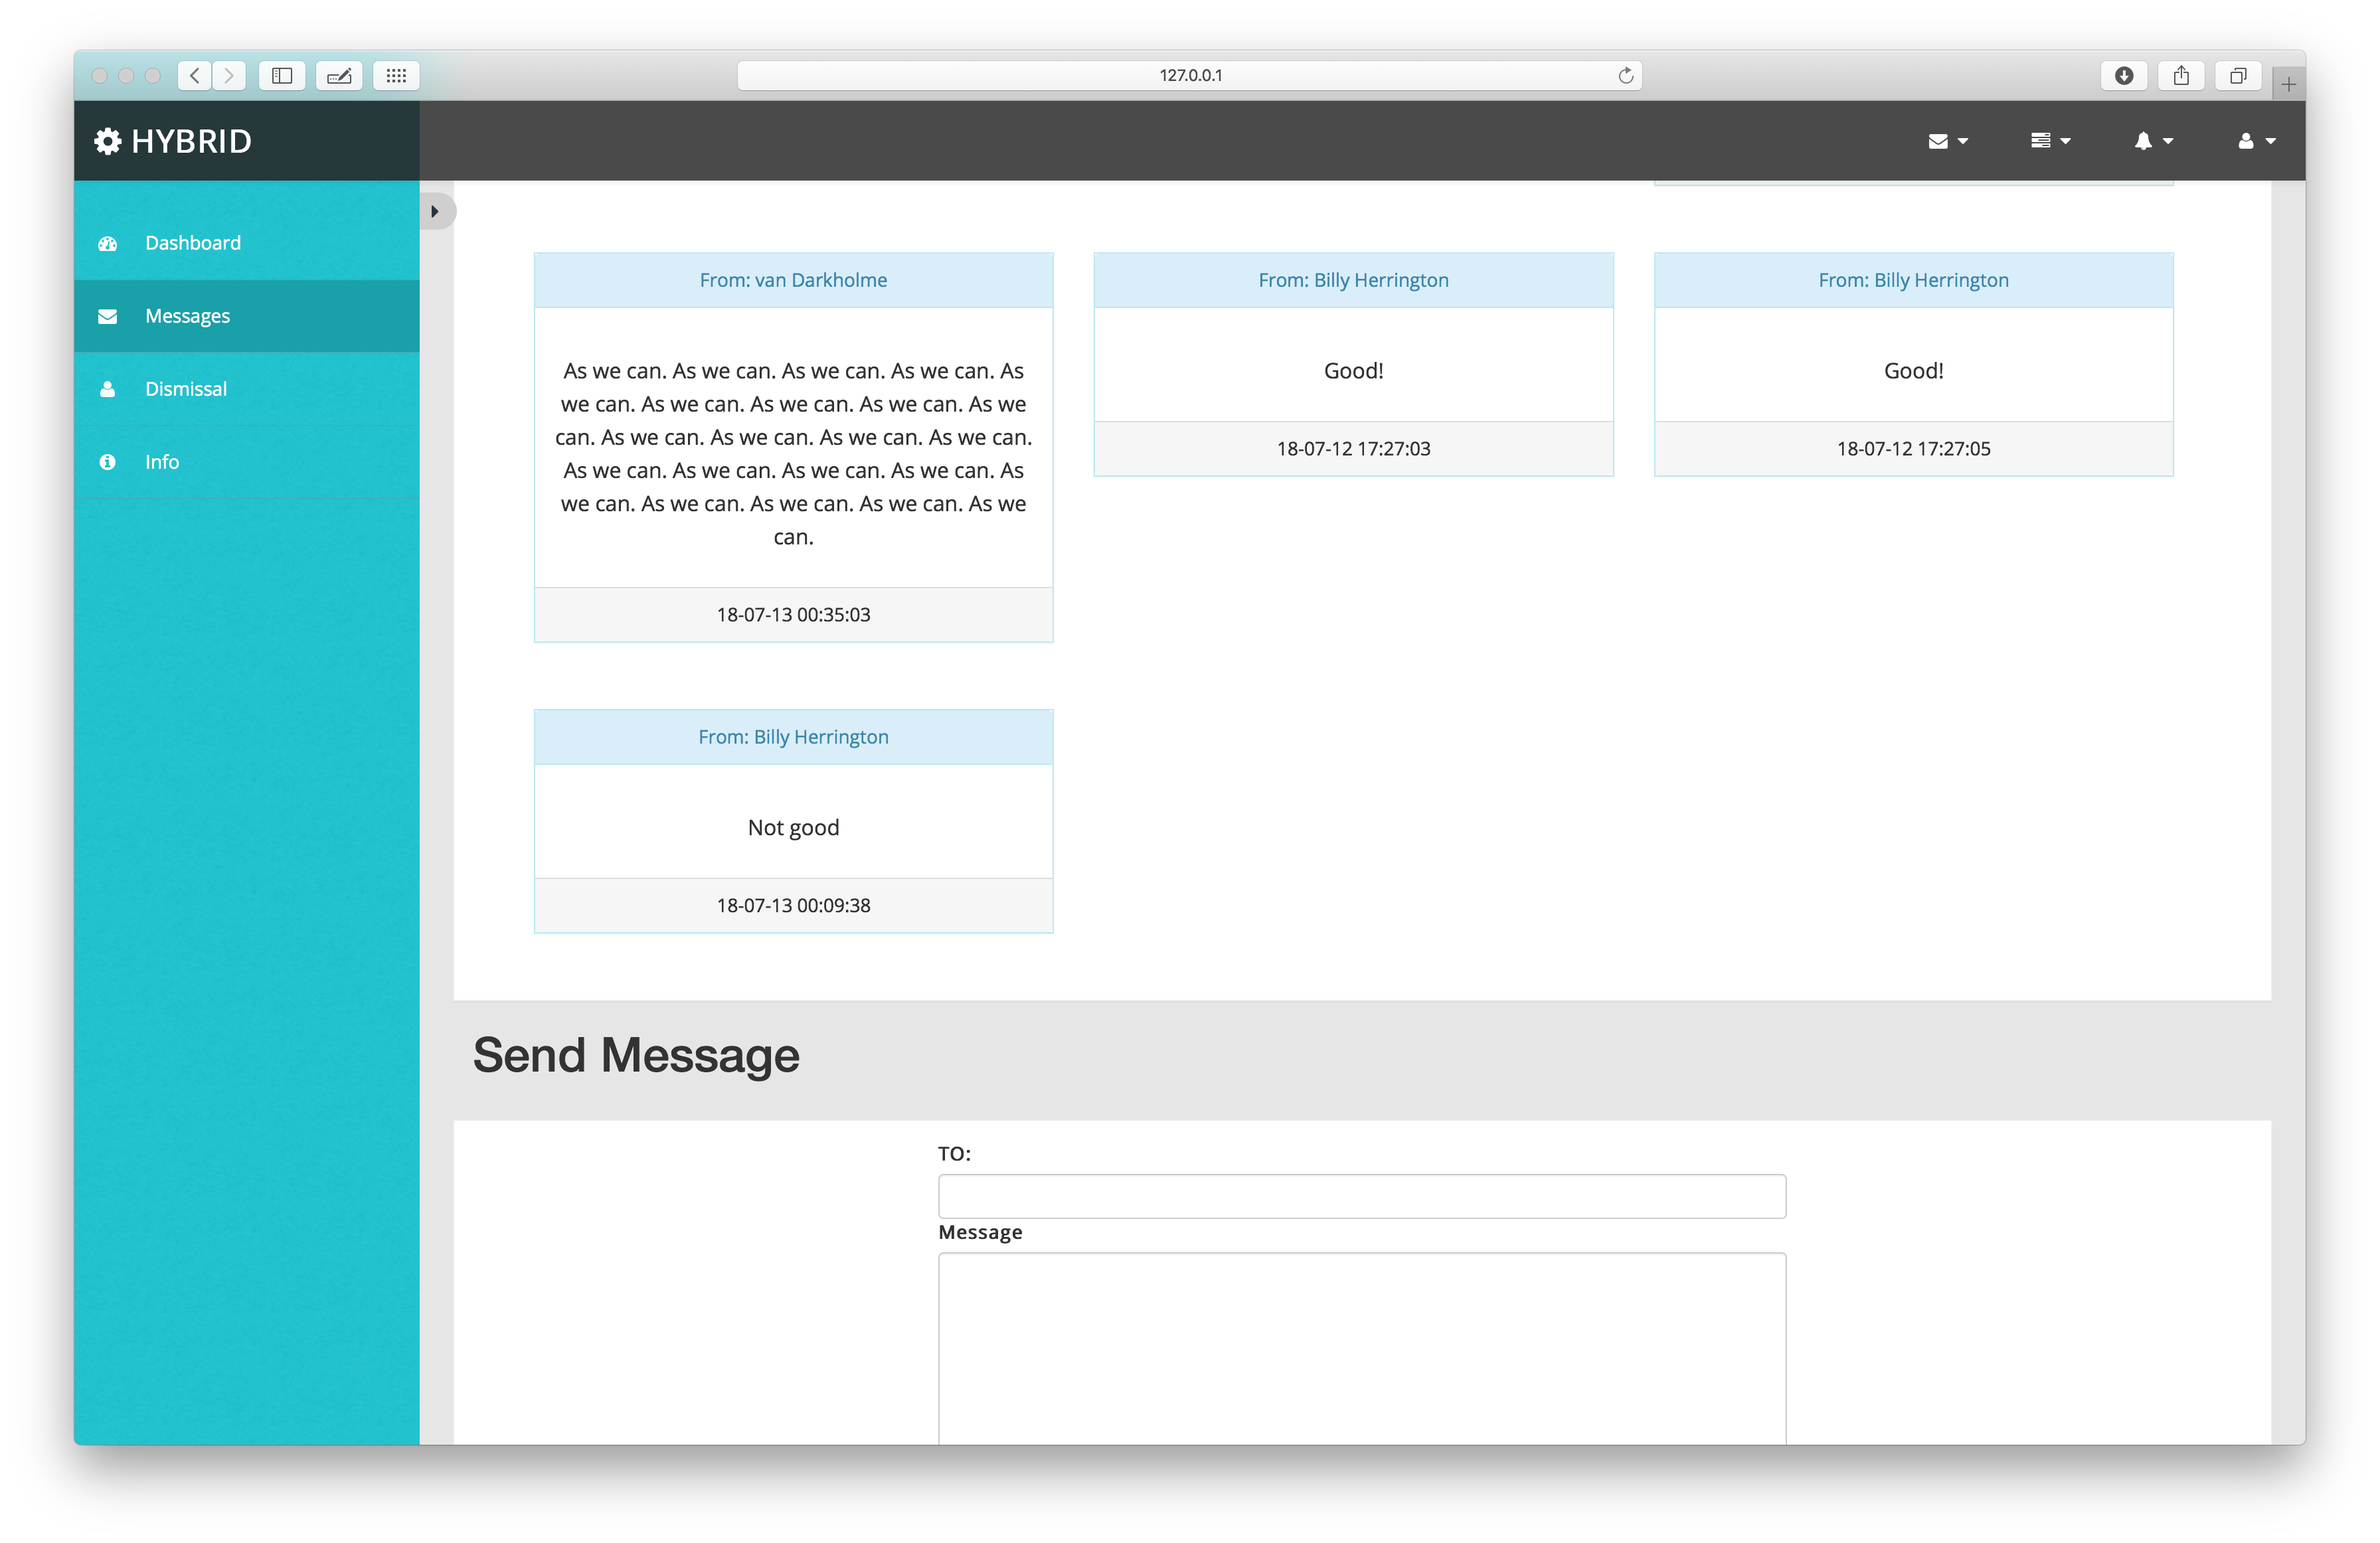
\includegraphics[width=\linewidth]{img/message2.png}
 		\caption{Web End}
 	\end{figure}

\subsection{Personal Information}
The personal information page shows the information of current user and his/her child. Information presented contains name, address, E-mail address, etc.
	\begin{figure}[H]
 	 \centering
 		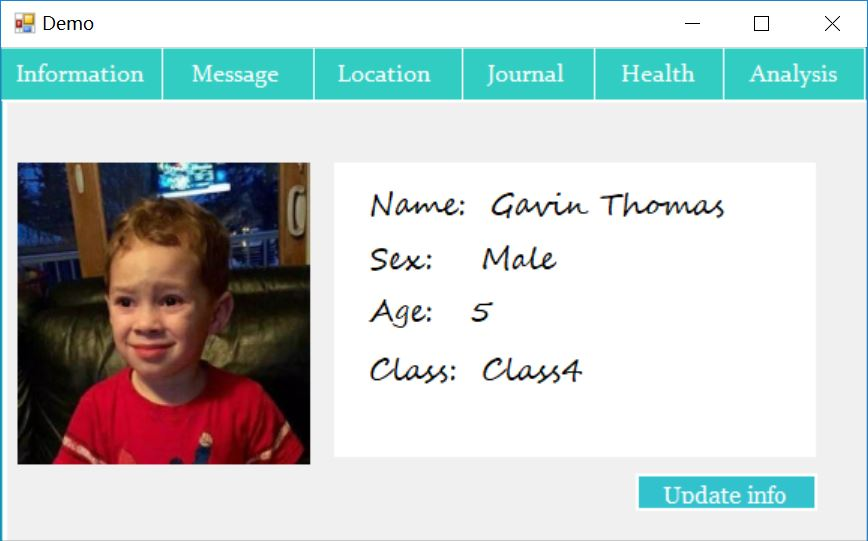
\includegraphics[width=0.8\linewidth]{img/information1.png}
 		\caption{PC End}
 	\end{figure}
 	\begin{figure}[H]
 	 \centering
 		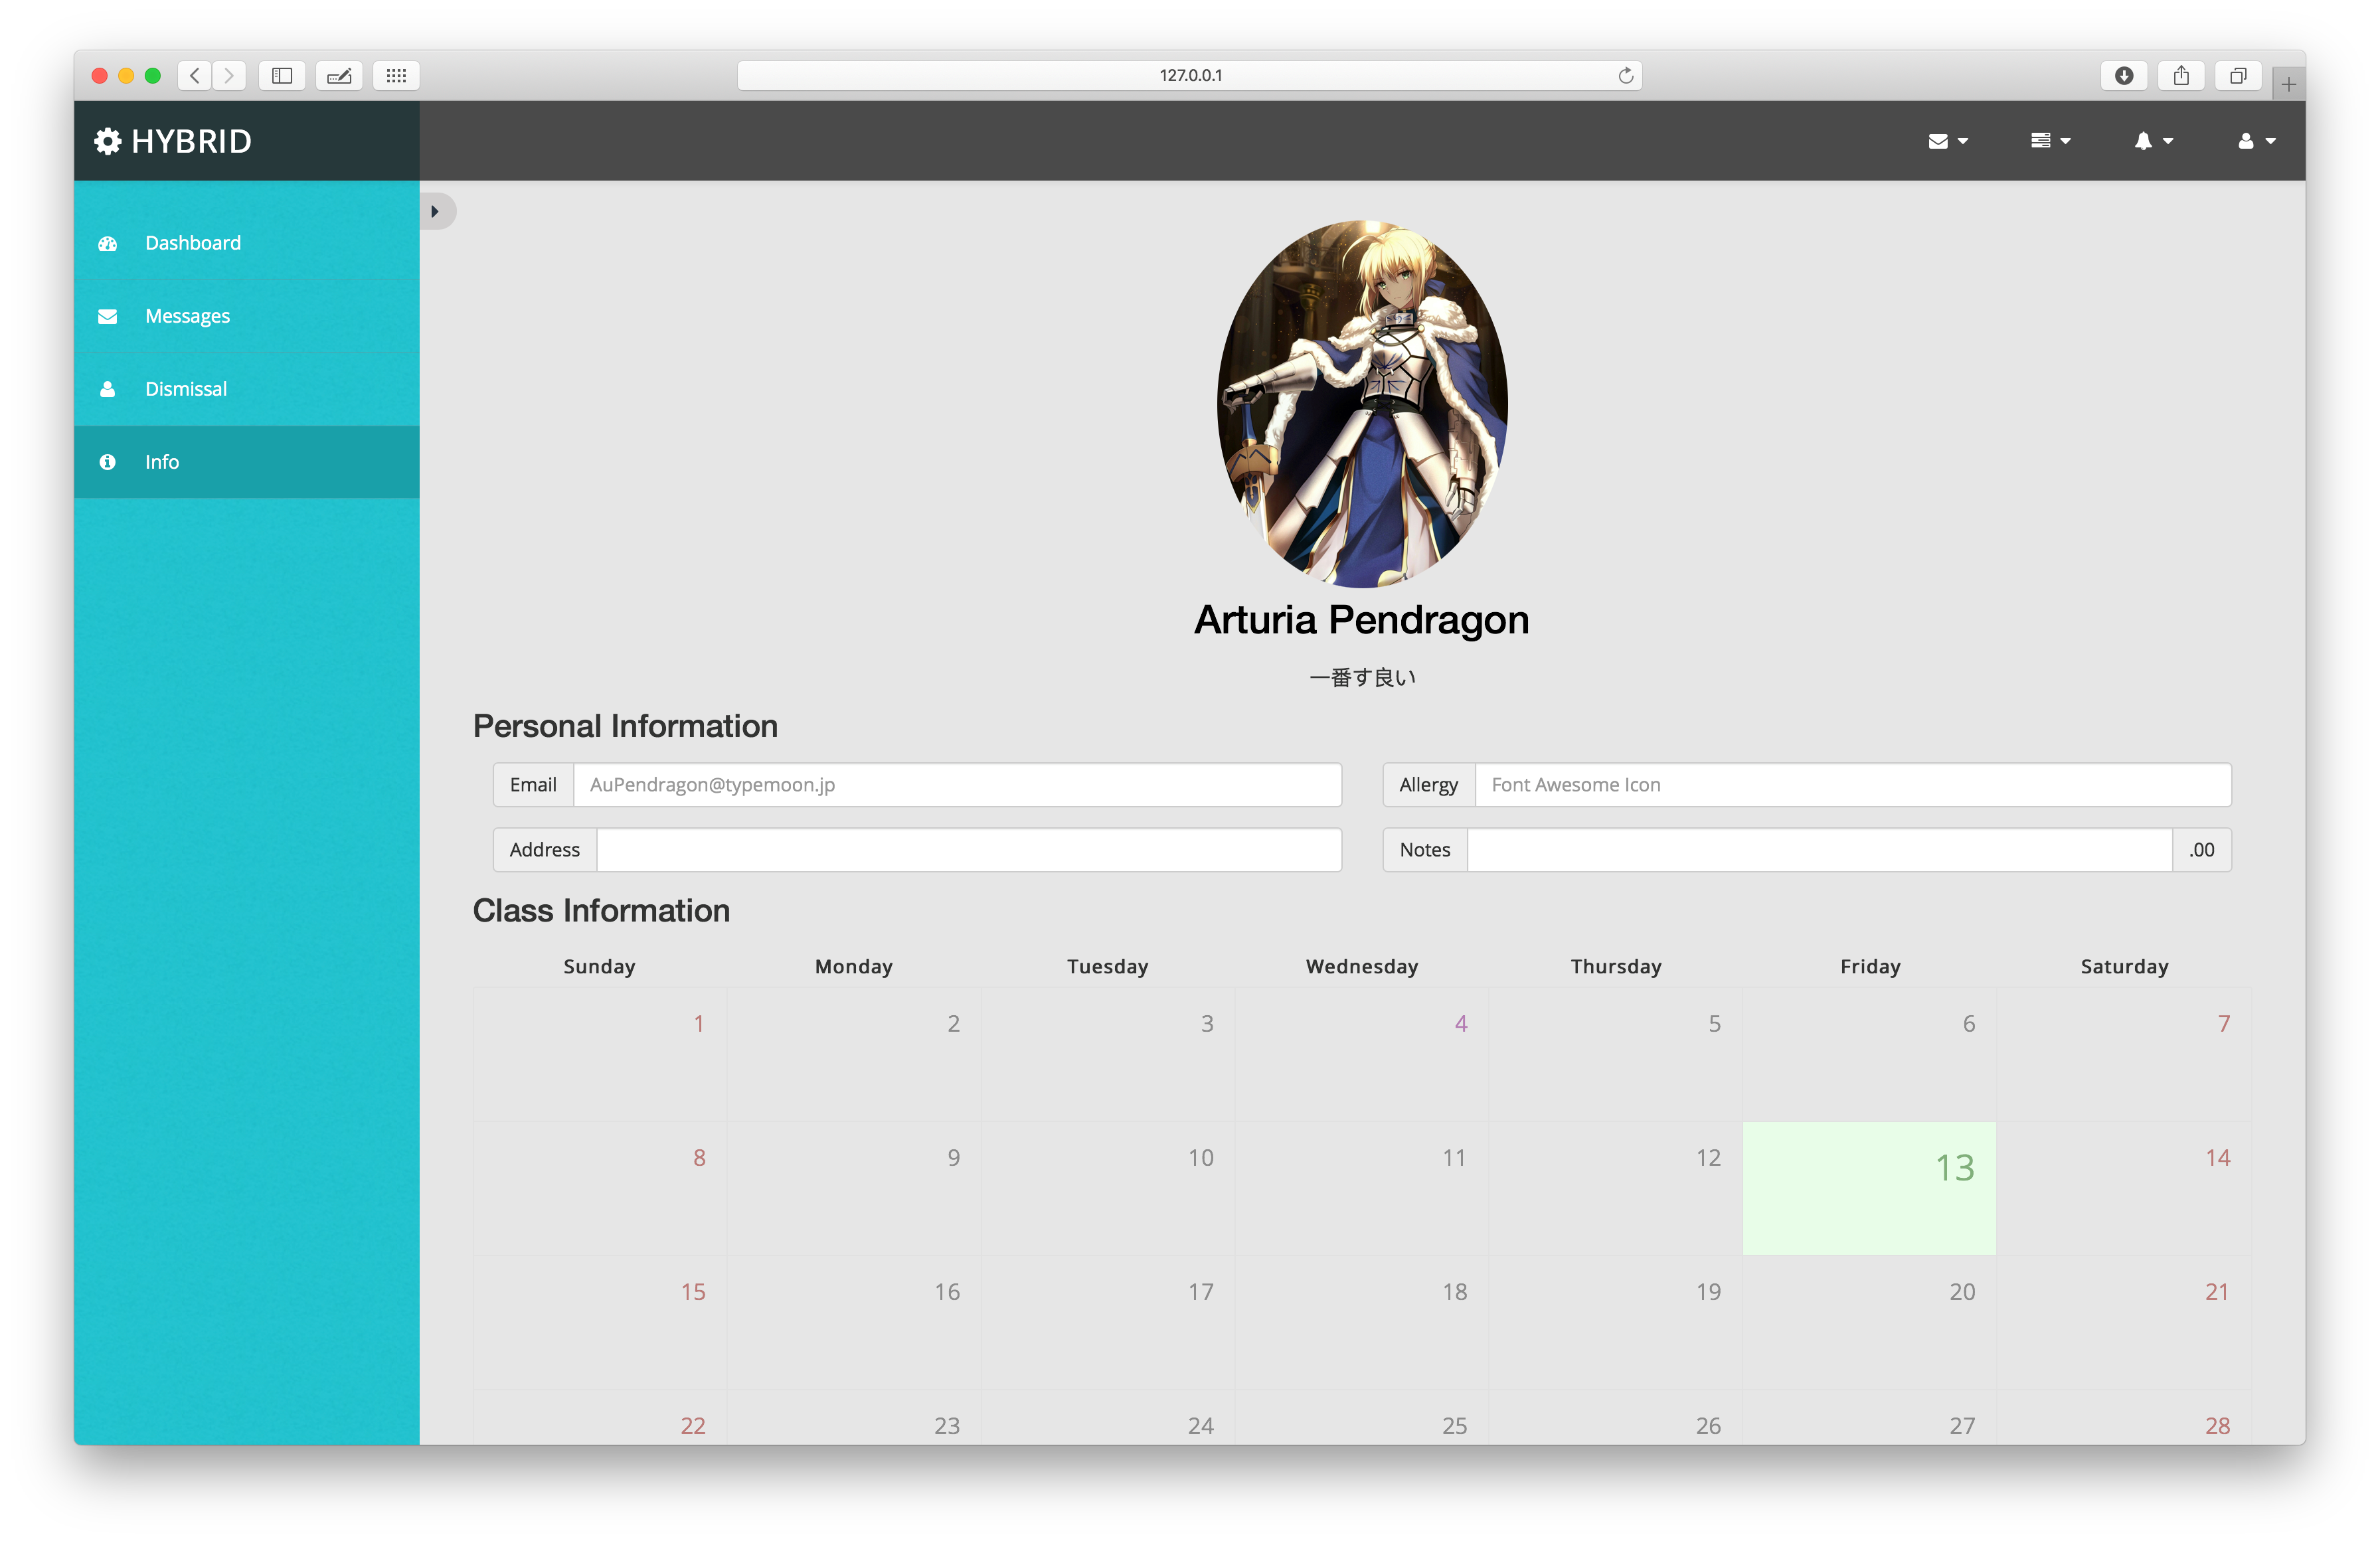
\includegraphics[width=\linewidth]{img/information2.png}
 		\caption{Web End}
 	\end{figure}

\section{Individual Contribution}
\subsection{Wanjun Xu}
\begin{itemize}
	\item Completed most part of the report
	\item Developed PC App
\end{itemize}

\subsection{Wenjia Liu}
\begin{itemize}
	\item Made group presentation
	\item Developed Android App
\end{itemize}

\subsection{Anjie Wang}
\begin{itemize}
	\item Revised report
	\item Set up local server 
	\item Developed backend for web app
\end{itemize}

\subsection{Hanxiang Ren}
\begin{itemize}
	\item Revise report
	\item Develop frontend for web app
\end{itemize}

\section{Lessons Learned}
This is the first time for us participating in this kind of class. Be aimed at solving a specific problem in real life, we are required to design a prototype and implement it by different groups’ cooperation. It’s a really fresh experience to everyone of us. \newline
The most significant problem we encountered is communication. Since our team does not work with data collected from sensor group directly, we think it's a better way for data analysis group, data visualization group, sensor to discuss format of each database. But, at the very beginning, this task was assigned to our group. and we failed to present our thoughts and concerns to HCI group, and that caused a lot trouble when cooperating with other group.


\end{document}